% Source: graduate-coursework/Prior_Semesters/Fa23/CSCE350/assignments/HW2_Backward_Substitution.tex

\documentclass[border=4pt]{standalone}
\usepackage{amsmath}
\usepackage{tikz}
\usetikzlibrary{arrows}

\begin{document}
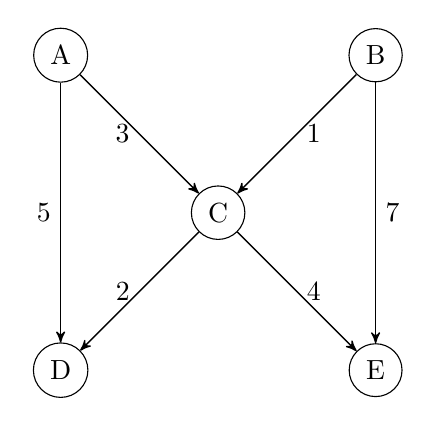
\begin{tikzpicture}[scale=2, > = latex'] % The 'latex'' option sets the arrowhead style
  \node[shape=circle,draw=black] (A) at (0,2) {A};
  \node[shape=circle,draw=black] (B) at (2,2) {B};
  \node[shape=circle,draw=black] (C) at (1,1) {C};
  \node[shape=circle,draw=black] (D) at (0,0) {D};
  \node[shape=circle,draw=black] (E) at (2,0) {E};
  
  \path [->, line width=0.5pt, >=stealth', scale=2] (A) edge node[midway, left] {3} (C);
  \path [->, line width=0.5pt, >=stealth', scale=2] (A) edge node[midway, left] {5} (D);
  \path [->, line width=0.5pt, >=stealth', scale=2] (B) edge node[midway, right] {1} (C);
  \path [->, line width=0.5pt, >=stealth', scale=2] (B) edge node[midway, right] {7} (E);
  \path [->, line width=0.5pt, >=stealth', scale=2] (C) edge node[midway, left] {2} (D);
  \path [->, line width=0.5pt, >=stealth', scale=2] (C) edge node[midway, right] {4} (E);
\end{tikzpicture}
\end{document}
